\documentclass[c]{beamer}
\usepackage{lmodern}% http://ctan.org/pkg/lm
\usepackage{amssymb}
\usepackage[utf8]{inputenc}
\usepackage{amsmath}
\usepackage{amsthm}
\usepackage{prftree}
\usepackage{graphicx}

% -- todo ------
\newcommand\todo[1]{\colorbox{blue!15}{\textbf{todo: }#1}\newline}
%\renewcommand\todo[1]{} % deactivate todos

\addtobeamertemplate{frametitle}{
   \let\insertframetitle\insertsectionhead}{}
\addtobeamertemplate{frametitle}{
   \let\insertframesubtitle\insertsubsectionhead}{}

\newtheoremstyle{break}
  {\topsep} {\topsep}%
  {}{}%
  {\bfseries}{:}%
  {\newline}{}%
\theoremstyle{break}

\title[] {AOTidF Bagger Game}
\author[Denis Erfurt, Tobias Behrens] % (optional, for multiple authors)
{Denis Erfurt, Tobias Behrens}

\begin{document}

  \frame{\titlepage} % Folie 1
  
  \section*{Agenda}
  \begin{frame}{title} % Folie 2
    \begin{enumerate}
      \item \textbf{Einführung}
      \begin{itemize}
        \item Aufgabenstellung
        \item Prämissen
        \item Forschungshypothesen
      \end{itemize}
      \item \textbf{theoretische Ergebnisse}
      \begin{itemize}
        \item Superadditivität
        \item NP-Härte
        \item Stabilisierung der großen Koalition
      \end{itemize}
      \item \textbf{praktische Ergebnisse}
      \begin{itemize}
        \item lineares Auktionsverfahren
        \item Ergebnisvergleich zum Shapley Value
      \end{itemize}
    \end{enumerate}
  \end{frame}
  
  
  \section*{Einführung}
  \subsection*{Aufgabenstellung}
  \begin{frame}{title} % Folie 3
    \todo{Aufgabenstellung}
    Aufteilung mit folgenden Eigenschaften:
    \begin{enumerate}
      \item soziale Wohlfahrt maximieren
      \item stabil
      \item fair
    \end{enumerate}
  \end{frame}


  \subsection*{Prämissen} 
  \begin{frame}{title} % Folie 4
    \begin{enumerate}
      \item Rationalität
      \item Multiskill
      \item Linearität des Verbrauchs
      \item unvollständige Information der Konkurrenz
      \item vollständige Informationen des Bedarfs
      \item Zeitagnostisch
    \end{enumerate}
  \end{frame}
  
  
  \subsection*{Allgemeine Forschungshypothesen}
  \begin{frame}{title} % Folie 5
    \begin{itemize}
      \item Das in der Aufgabenstellung beschriebene Zuordnungsproblem ist superadditiv  und erfordert einen NP-harten Mechanismus.
      \item Die große Koalition als Lösungsstrategie mit Shapley Value als  Auszahlungsvorschrift ist instabil. Wir können eine Erweiterung vorschlagen, um eine stabile große Koalition zu erhalten.
      \item Es existiert ein lineares Auktionsverfahren, das eine Zuordnung untern den Vorgaben approximiert.
    \end{itemize}
  \end{frame}


  \section*{theoretische Ergebnisse}
  \subsection*{Superadditivität}
  \begin{frame}{title} % Folie 6
    \todo{Superadditivität}
    \begin{lemma}[Superadditivität von CSG]
      Das CSG ist Superadditiv.
    \end{lemma}
  \end{frame}
  
  
  \subsection*{NP-Härte}
  \begin{frame}{title} % Folie 8
    \todo{NP-Härte}
    \begin{lemma}[NP-Härte des Problems]
    
    \end{lemma}
  \end{frame}
  
  
  \subsection*{Stabilisierung der großen Koalition}
  \begin{frame}{title} % Folie 9
    \begin{lemma}[Instabilität]
      Im allgemeinen Fall ist die große Koalition $K=Agenten$ instabil.  
    \end{lemma}

      \begin{figure}
        \centering
        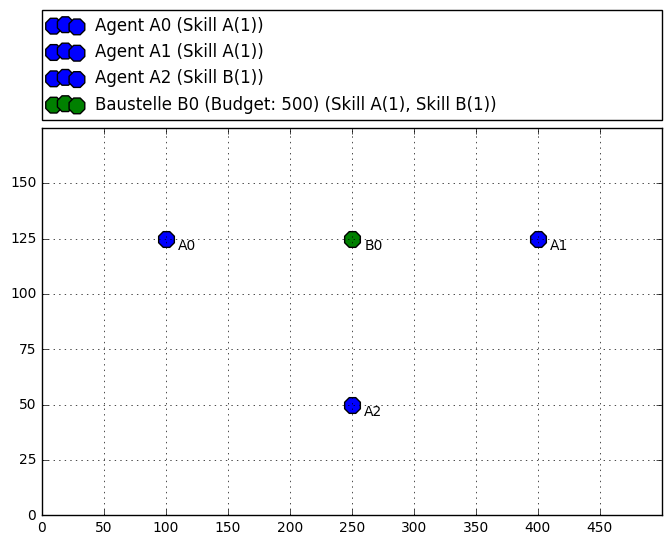
\includegraphics[width=0.6\textwidth]{example-exchangeable-agents.png}
        \label{szenario1}
      \end{figure}

  % Der Gewinn der Koalitionen $K_1 = \{A0, A1, A2\}$ und $K_2 = \{A0, A2\}$ ist gleich, jedoch erhält die Agenten $A0$ in $K_2$ anteilig mehr vom Gewinn. Demnach lohnt es sich für ihn die große Koalition zu verlassen.
  \end{frame}
  \begin{frame}{title} % Folie 10
    \todo{Stabilisierung der großen Koalition}
  \end{frame}
  

  \section*{praktische Ergebnisse}
  \subsection*{lineares Auktionsverfahren}
  \begin{frame}{title}
    sequentielle Rückwärtsauktion $\forall{b \in Baustellen}$:
    \begin{enumerate}
      \item Ausschreibung der gesuchten Skilltypen
      \item alle Agenten können auf einen oder mehrere Skilltypen bieten
      \item das niedrigste Gebot erhält den Zuschlag \\[2em]
    \end{enumerate}
    
    Die Auszahlung an gewinnende Agenten anhand ihres Gebotes:
    \begin{itemize}
      \item Auszahlung des Gebotes
      \item verbliebener Erlös der Baustelle in Abhängigkeit zu dem Anteil eines Gebotes an der Gesamtgebotsumme
    \end{itemize}
  \end{frame}
  
  \subsection*{Ergebnisvergleich zum Shapley Value}
  \begin{frame}{title}
    \textbf{Vorgehen}
    \begin{enumerate}
      \item Generierung von Testszenarien
      \item für jedes Szenario: beste Zuordnung aller möglichen Koalitionen bestimmen und Auszahlung nach Shapley Value berechnen
      \item Auktionsverfahren für jedes Szenario simulieren
      \item Vergleich der Auszahlungsergebnisse im Hinblick auf den Gewinn der Agenten
    \end{enumerate}
  \end{frame}
  
  \begin{frame}{title}
    \textbf{Ergebnisse}
    \begin{figure}
      \centering
      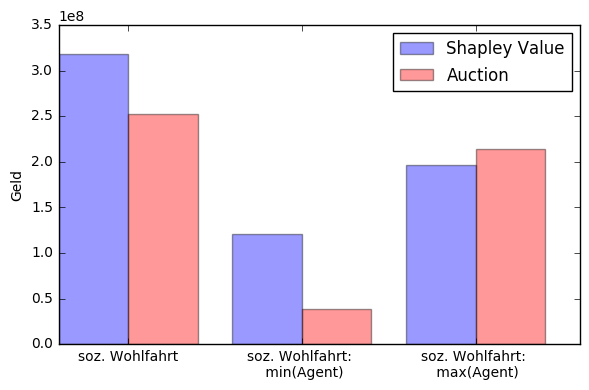
\includegraphics[width=0.8\textwidth]{results.png}
    \end{figure}
    \todo{weitere Auswertungen}
  \end{frame}


\end{document}